\begin{figure}[h!]
\vspace*{-1.5cm}
\centering
\definecolor{ttttff}{rgb}{0.2,0.2,1}
\definecolor{qqqqff}{rgb}{0,0,1}
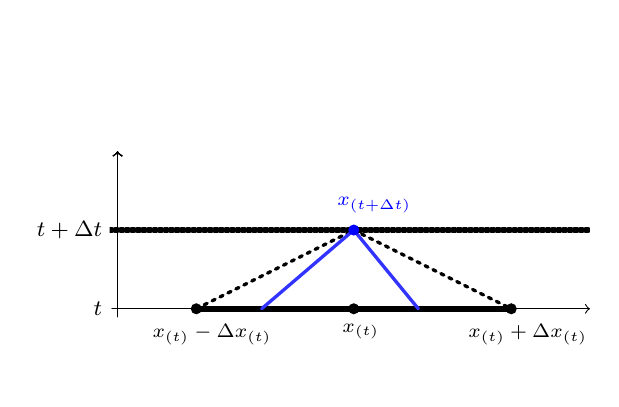
\begin{tikzpicture}[line cap=round,line join=round,x=1cm,y=1cm]
\draw[->,color=black] (1,0) -- (7,0);
\foreach \x in {1,2,3,4,5,6,7}
\draw[->,color=black] (1,-0.1) -- (1,2);
\draw[shift={(1,0)},color=black] (2pt,0pt) -- (-2pt,0pt) node[left] {\footnotesize ${t}$};
\draw[shift={(1,1)},color=black] (2pt,0pt) -- (-2pt,0pt) node[left] {\footnotesize $t + \Delta t$};
\clip(0.9,-0.89) rectangle (7,3.57);
\draw [line width=2pt,dash pattern=on 1pt off 1pt,domain=-0.37:7.9] plot(\x,{(--4-0*\x)/4});
\draw [line width=2pt] (2,0)-- (4,0);
\draw [line width=2pt] (4,0)-- (6,0);
\draw [line width=1.2pt,dotted] (2,0)-- (4,1);
\draw [line width=1.2pt,dotted] (4,1)-- (6,0);
\draw [line width=1.2pt,color=ttttff] (4,1)-- (4.82,0);
\draw [line width=1.2pt,color=ttttff] (4,1)-- (2.83,0);
\begin{scriptsize}
\fill [color=black] (2,0) circle (2pt);
    \draw[color=black] (2.2,-0.1) node[below] {$x_{(t)} - \Delta x_{(t)}$};
\fill [color=black] (4,0) circle (2pt);
    \draw[color=black] (4.09,-0.09) node[below] {$x_{(t)}$};
\fill [color=black] (6,0) circle (2pt);
    \draw[color=black] (6.21,-0.1) node[below] {$x_{(t)} + \Delta x_{(t)}$};
\fill [color=qqqqff] (4,1) circle (2pt);
    \draw[color=qqqqff] (4.26,1.12) node[above] {$x_{(t + \Delta t)}$};
\end{scriptsize}
\end{tikzpicture}
    
    \caption{CFL, spatial and temporal stencils.}
    \label{fig:CFL}

\end{figure}
